\chapter{Introducción al cálculo simbólico\\Introduction to symbolic computing}\index{Cálculo Simbolico}\index[eng]{Symbolic Computing}
\chaptermark{Intro cálculo simbólico  \textreferencemark\ Intro symbolic computing}
\epigraph{And earthly power doth then show likest God's
	when mercy seasons justice.}{The merchan of Venice, Willian Shakespeare}
\begin{flalign*}
	&\mathwitch*_{i=0}^{\infty}\Biggl \{&     
\end{flalign*}
\begin{paracol}{2}
En este último capítulo vamos a introducir un método de cálculo que difiere notablemente de lo visto  en los capítulos anteriores: se trata del cálculo simbólico. Hasta ahora, hemos empleado siempre el ordenador para hacer cálculo numérico. Las variables se definían asignándoles un valor numérico y después eran empleadas en operaciones algebraicas o se les aplicaban funciones matemáticas para obtener a partir de ellas resultados numéricos.

Sin embargo, en matemáticas y en física, es práctica habitual realizar operaciones con variables y funciones sin asignarles un resultado numérico. Un ejemplo típico es el de la derivación de una función,
\switchcolumn
In this last chapter we are going to introduce a computing method completely different to the method described in previous chapters: Symbolic computing. So far, we have always use the computer to perform numerical computing. Variables were defined assigning them a numerical value a after, they were used in algebraic operations of introduced in functions to obtain numerical results.

Nevertheless, in mathematics and physics, it is common practice to perform operations with variables and function without assign to them numerical results. A classic example is function derivation, 
\end{paracol}
\begin{equation*}
f(x) = \sqrt{1-\ln x} \rightarrow f'(x) =-\frac{1}{2x\sqrt{1 - \ln x}} 
\end{equation*}  
\begin{paracol}{2}
A partir de una expresión \emph{simbólica} de la función obtenemos su derivada expresada también de modo \emph{simbólico} como otra función. También con un computador es posible hacer este tipo de operaciones, a las que se da el nombre de cálculo simbólico para distinguirlas del cálculo numérico.
\switchcolumn
Departing from a function \emph{symbolic} expression, we get its derivative also expressed in a \emph{symbolic} way. This process can also be performed using a computer, which is referred to as symbolic computing, distinguishing it from numerical computing. 
\end{paracol}

\begin{paracol}{2}
\section{Cálculo simbólico con Sympy}
\sectionmark{Calculos simbólico con Sympy. \textreferencemark\ Symbolic computing with Sympy.}
Sympy  es un módulo de Python creado para realizar cálculo simbólico. Como en el caso de otros módulos que hemos introducido en capítulos anteriores, nos vamos a limitar a dar una introducción al cálculo simbólico empleando Sympy, para conocer de verdad sus posibilidades se aconseja acudir a la documentación del módulo, disponible en Internet.

\section{Variables y expresiones simbólicas}
\sectionmark{Var. y expr. simbólicas. \textreferencemark\ Symbolic var. and expr.}
\subsection{Variables simbólicas} \index{Variable! Simbólica}
Una variable simbólica, a diferencia de las variables ordinarias de Python, no contiene un valor; simplemente es un objeto que puede manipularse empleando reglas  algebraicas ordinarias. Importamos el módulo del mismo modo que cualquier otro módulo de Python. Para crear una variable simbólica, se emplea el comando \mintinline{python}|symbols|,
\switchcolumn

\section{Symbolic computing with Sympy }
Sympy is a Python's module created to perform symbolic computing. As in other modules we have introduced in previous chapters, we are going to limit our exposition to give an introduction to symbolic computing using Sympy. To truly know its capacity, it is advisable to check the module documentation, available in Internet.

\section{Variables and symbolic expressions}
\subsection{Symbolic variables} \index[eng]{Variable! Symbolic}
In contrast to a standard Python variable, a symbolic variable doesn't have a value. It is just an object that can be manipulated using ordinary algebraic rules. To import the Sympy module, we proceed in the same way as with other Python modules. To create a symbolic variable, we use the command \mintinline{python}|symbols|,


\end{paracol}
\begin{center}
	\begin{minipage}{.3\textwidth}
		\begin{minted}{python}
In [1]: import sympy as sp
In [2]: x,y = sp.symbols('x y')
In [3]: x
Out[3]: 
x
In [4]: y
Out[4]: 
y
In [5]: z = sp.symbols('x')
In [6]: z
Out[6]: 
x				
		\end{minted}
	\end{minipage}
\end{center}
\begin{paracol}{2}
Así, el comando asigna a las variables que definamos separadas por comas a la izquierda del igual, los símbolos, separados por espacios y encerrados entre comillas simples, introducidos a \mintinline{python}|symbols()|.

Cuando pedimos a Python que nos muestre el contenido de la variable \texttt{x} nos indica que contiene el símbolo \texttt{x}. Es importante remarcar que aquí no se trata de un caracter sino de un símbolo con el que se pueden realizar operaciones algebraicas y que el nombre de la variable que contiene el símbolo no tiene porqué coincidir con este. Así, por ejemplo, a la variable \texttt{z}, le hemos vuelto a asignar el simbolo \texttt{x}.

También es posible crear vectores y matrices simbólicas a partir de otras variables simbólicas,
\switchcolumn
Thus, the command assigns the variables on the left of the equal sign, split by commas, the symbols provided in \mintinline{python}|symbols()|, which are divided by spaces and enclosed in apostrophes.

When we ask Python to display the value of the variable \texttt{x}, it points out that the variable holds the symbol \texttt{x}. It is important to remark that it is not a character but a symbol that we can use to perform algebraical operations and that the name of the variable that holds a symbol is not necessarily the symbol itself. For instance, in the example, we have reassigned the symbol \texttt{x} to variable \texttt{z}

It is also possible to create symbolic vectors and matrices from other symbolic variables,

\end{paracol}
\begin{center}
	\begin{minipage}{.5\textwidth}
		\begin{minted}{python}
In [25]: from sympy import matrices as mt
In [26]: a,b,c = sp.symbols('a b c')
In [27]: A = mt.Matrix([[a,b,c],[c,b,b],[a,c,a]])
			
In [28]: A
Out[28]: 				
		\end{minted}
\[
\begin{bmatrix}
a&b&c\\
c&b&b\\
a&c&a
\end{bmatrix}
\]
	\end{minipage}
\end{center}
\begin{paracol}{2}
Los comandos y funciones más habituales asociados a los arrays de numpy funcionan con las matrices de Sympy. Por ejemplo podemos extraer elementos o filas de una matriz, calcular el determinate o la inversa,
\switchcolumn
Most common comand and function defined for Numpy arrays work also with Sympy matrices. For instance, we can extract elements of rows from a matrix, compute the determinant of the inverse matrix, 
\end{paracol}
\begin{center}
	\begin{minipage}{.5\textwidth}
		\begin{minted}{python}
In [44] A[0,0]
Out[44]: 
\end{minted}
$a$	 				
\begin{minted}{python}
In [48]: A[1,:]
Out[48]:
\end{minted}
$[c,b,b]$
\begin{minted}{python}
In [46]: A.det()
Out[46]: 
\end{minted}
$a^2b+ab^2-3abc+c^3$
\end{minipage}
\end{center}
\begin{center}
	\begin{minipage}{.5\textwidth}

\begin{minted}{python}
In [50]: A.inv()
Out[50]: 
\end{minted}
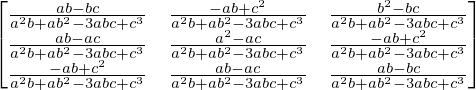
\includegraphics[width=1.4\textwidth]{inversa_m.png}
	\end{minipage}
\end{center}
\begin{paracol}{2}
Otra opción posible es crear un objeto simbolico matriz. La idea es crear una variable simbólica que contiene una matriz del tamaño que deseemos. Para ello empleamos el comando \mintinline{python}|MatrixSymbol|de \mintinline{python}|sympy.matrices|. Este comando admite un símbolo y dos parámetros numéricos que corresponden con el número de filas y columnas de la matriz creada. Estos parámetros tambień podrían a su vez ser simbólicos.
\switchcolumn
An alternative is to create a symbolic matrix object. We make a symbolic variable that holds a matrix the size we wish. The command \mintinline{python}|MatrixSymbol| from \mintinline{python}|sympy.matrices| allows to make a symbolic matrix. This command takes a symbol and two numerical parameters which define the number of rows and columns of the matrix we are creating. In fact, these two last parameter could be also symbolic.
\end{paracol}
\begin{center}
	\begin{minipage}{.3\textwidth}
		\begin{minted}{python}
In [56]: B = mt.MatrixSymbol('b',3,3)
B.shape
Out[60]: (3, 3)				
		\end{minted}
	\end{minipage}
\end{center}
\begin{paracol}{2}
Podemos obtener a partir de un objeto matriz simbólico la matriz simbólica de forma explícita,
\switchcolumn
We can get explicitly the symbolic matrix from a symbolic matrix object,
\end{paracol}
\begin{center}
	\begin{minipage}{.3\textwidth}
\begin{minted}{python}
In [70]: B.as_explicit()
Out[70]:				
\end{minted}
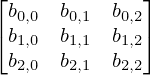
\includegraphics[width=0.8\textwidth]{matrixexp.png}		
	\end{minipage}
\end{center}
\begin{paracol}{2}
y también aplicar operaciones matriciales, sobre las formas explícitas,
\switchcolumn
and then, to apply matrix operations to the explicit matrices.
\end{paracol}
\begin{center}
\begin{minipage}{.8\textwidth}
	\begin{minted}{python}
		In [23]: B.as_explicit().det()
		Out[23]:			
	\end{minted}
	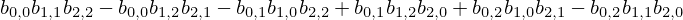
\includegraphics[width=1.1\textwidth]{detsimbol.png}		
\end{minipage}
\end{center}

\begin{paracol}{2}
\subsection{Expresiones simbólicas}
Podemos ahora realizar operaciones aritméticas, con nuestras variables simbólicas,
\switchcolumn
\subsection{Symbolic expressions}
We can now perform arithmetical operations with our symbolic variables,
\end{paracol}
\begin{center}
\begin{minipage}{.5\textwidth}
	\begin{minted}{python}
In [12]: q = 2*z + 2*x -y
In [13]: q
Out[13]: 			
	\end{minted}
	$4x - y$
\end{minipage}
\end{center}

\begin{paracol}{2}
El resultado es en este caso una expresión que guarda el resultado de la operación realizada. Es interesante notar cómo Sympy ha operado el contenido simbólico de las variables \texttt{x} y \texttt{z} para dar como resultado $4x$.

Para crear expresiones más complejas, Sympy tiene definidas las funciones matemáticas más comunes como funciones simbólicas,
\switchcolumn
The result now is an expression that holds the result of the operation we have carried out. It is interesting to note how Sympy operates the symbolic values of variables \texttt{x} and texttt{z} to cast the result $4x$. 

SymPy has the most common mathematical functions defined as symbolic functions, enabling the creation of more complex expressions.
\end{paracol}

\begin{center}
\begin{minipage}{.8\textwidth}
	\begin{minted}{python}
In [23]: expr = sp.cos(x)**2 + sp.sqrt(y) + sp.exp(x**2)
In [24]: expr
Out[24]: 			
	\end{minted}
	$\sqrt{y}+e^{x^2}+\cos^2(x)$
\end{minipage}
\end{center}

\begin{paracol}{2}
En el siguiente ejemplo, se han creado primero cuatro variables simbólicas y, a partir de ellas, se han generado tres expresiones simbólicas, la primera es un polinomio de grado dos y las dos siguientes las expresiones analíticas de sus raíces.
\switchcolumn
The following example illustrates how to define four symbolic variables and construct three symbolic expressions from them. The first expression is a degree two polynomial, and the subsequent two are its roots analytic expressions.

\end{paracol}
\begin{center}
\begin{minipage}{.5\textwidth}
	\begin{minted}{python}
In [14]: a,b,c,x =sp.symbols('a b c x')

In [15]: y = a*x**2+b*x+c

In [16]: rp = (-b+sp.sqrt(b**2-4*a*c))/(2*a)

In [17]: rn = (-b-sp.sqrt(b**2-4*a*c))/(2*a)
	\end{minted}
\end{minipage}
\end{center}
\begin{paracol}{2}
Es posible definir funciones de más de una variable,
\switchcolumn
It is possible to define functions with several variables
\end{paracol}
\begin{center}
	\begin{minipage}{.5\textwidth}
		\begin{minted}{python}
In [22]: x,y,z =sp.symbols('x y z')
			
In [23]: f = sp.sin(x)**2+sp.cos(x)**2
In [24]: f
Out[24]: 
		\end{minted}
		$f = \sin^2(x) + \cos^2(x)$
	\end{minipage}
\end{center}

\begin{paracol}{2}
o también, combinar funciones simbólicas mediante operadores aritméticos o composición de funciones,
\switchcolumn
and also, combine symbolic functions by mean of arithmetic operator or function composition
\end{paracol}
 
\begin{center}
	\begin{minipage}{.25\textwidth}
		\begin{minted}{python}
In [25]: g= 1/z**2
In [26]: fg = f*g
In [27]: fg
Out[28]:
		\end{minted}
	\end{minipage}
	\begin{equation*}
		fg = \frac{\sin^2(x) + \cos^2(x)}{z^2}
	\end{equation*}
\end{center}
\begin{paracol}{2}
\subsection{Simplificación de expresiones simbólicas}
Sympy permite, dada una expresión simbólica, obtener una equivalente más sencilla. En general, este proceso de simplificación no es trivial ni unívoco, ya que una expresión puede admitir varias formas simplificadas. Es también posible que la expresión simbólica que deseamos simplificar, no sea simplificable.

Es interesante, sobretodo cuando se trata de expresiones obtenidas a partir de cálculos simbólicos, tratar de obtener una expresión lo más simplificada posible. La razón es que resulta mucho más fácil de entender y manipular. Sympy suministra el comando \texttt{simplify} para simplificar expresiones simbólicas. Así por ejemplo, si aplicamos \texttt{simplify} a la expresión \texttt{f\_g}, que acabamos de definir en la sección anterior, 
\switchcolumn
\subsection{Symbolic expression simplification}
SymPy can take a symbolic expression and generate an equivalent, simplified version. However, this process is not always straightforward or unique, as an expression may have multiple valid simplified forms. Additionally, it's possible that the expression we wish to simplify cannot be simplified at all.

It is interesting, mainly when we get an expression using symbolic computing, try to simplify it as much as possible. Obviously, the simplified version is easier to understand and manipulate. Sympy supplies the command \texttt{simplify} to simplify symbolic expressions. For instance, if we apply the command \texttt{simplify} to the expression \texttt{f\_g}we have just obtained in the previous section,
\end{paracol}
\begin{center}
	\begin{minipage}{.25\textwidth}
		\begin{minted}{python}
In [33]: sp.simplify(f_g)
Out[33]: 
		\end{minted}
	\end{minipage}
	\begin{equation*}
		fg = \frac{1}{z^2}
	\end{equation*}
\end{center}
\begin{paracol}{2}
Obtendremos un $1$ en el numerador, como cabría esperar. Este ejemplo es particularmente simple y, aunque sirve para ilustrar el funcionamiento del comando, no siempre es posible conseguir soluciones tan satisfactorias.

Veamos otro ejemplo que muestra la ambigüedad del comando \texttt{simplify},

\switchcolumn
We obtain 1 in the numerator, which is expected. This is a straightforward example that illustrates the command's performance, though it may not always yield such satisfactory results.

Let's see another example that shows the ambiguity of the \texttt{simplify} command,
\end{paracol}
\begin{center}
	\begin{minipage}{.25\textwidth}
		\begin{minted}{python}
In [37]: bn = x**2+2*x*y+y**2
In [38]: sp.simplify(bn)
Out[38]:
		\end{minted}
		$x^2+2xy+y^2$
	\end{minipage}
\end{center}
\begin{paracol}{2}
En este caso, Sympy devuelve la misma expresión que hemos introducido. Podríamos preguntarnos si no debería devolver la expresión como un binomio $(x+y)^2$. La cuestión es hasta qué punto podemos consider que esta expresión es más simple que la original. Para evitar algunas ambigüedades de este tipo, Sympy tiene varios comando para 'simplificar' expresiones. Por ejemplo, la función \mintinline{Python}|factor|, nos permite realizar la transformación deseada en el ejemplo anterior,

\switchcolumn
In this case, SymPy retrieves the same expression that we provided to the command. The question arises: should it retrieve the expression as a binomial, \((x+y)^2\)? Can we consider this binomial to be simpler than the original expression? To avoid such ambiguities, SymPy offers several commands to simplify expressions. For example, the function `factor` allows us to perform the desired transformation for the previous example.
\end{paracol}
\begin{center}
	\begin{minipage}{.25\textwidth}
\begin{minted}{python}
In [44]: bnf = sp.factor(bn)
In [45]: bnf
Out[45]:
\end{minted}
$(x+y)^2$

\begin{minted}{python}
In [46]: sp.expand(bnf)
Out[46]:
\end{minted}
$x^2+2xy+y^2$
\end{minipage}
\end{center}
\begin{paracol}{2}
Comos se muestra en la línea [46] es posible tambíen desarrollar una expresión binomial, para obtener un polinomio, empleando la función \mintinline{python}|expand|. En nuestro ejemplo, esto revertiría la acción de \mintinline{python}|factor|.
\switchcolumn
As can be seen in line [46], it is also possible to expand a binomial expression into a polynomial, using the \mintinline{python}|expand| function. In our case, this reverts the actions of the command \mintinline{python}|factor|.
\end{paracol}

\begin{paracol}{2}
\subsection{Sustitución de variables y expresiones.}
Es posible, una vez definida una expresión simbólica, sustituir sus variables por otras expresiones empleando el comando \texttt{subs}. La sintáxis es simple, tomamos el nombre de la variable en que guardamos la expresión simbólica que queremos modificar, invocamos el método \texttt{subs}, indicando el nombre de la variable simbólica que queremos substituir y la expresión por la que queremos sustituirla. 

Por ejemplo podemos cambiar en la expresión $(x+y)^2$ que creamos anteriormente, la variable x por la variable z\footnote{Solo se pueden emplear variables simbólicas previamente definidas para hacer la sustitución}. 
\switchcolumn
\subsection{Substituting variables and expressions.}
Once a symbolic expression has been defined, you can substitute its variables with other expressions using the command \texttt{subs}. The syntax is simple: you specify the name of the variable that holds the symbolic expression you want to modify, call the command \texttt{subs}, and indicate the name of the symbolic variable you wish to substitute along with the expression you want to use in its place. 

For example, if we take the expression \((x+y)^2\) that we created earlier, we can replace the variable \(x\) with the variable \(z\)\footnote{Note that only previously defined symbolic variables can be used for substitution.}.

\end{paracol}
\begin{center}
	\begin{minipage}{.25\textwidth}
		\begin{minted}{python}
In [50]: bnf.subs(x,z)
Out[50]:
		\end{minted}
		$(y+z)^2$
	\end{minipage}
\end{center}

\begin{paracol}{2}
También podemos sustituir una expresión simbólica por un número, aunque es importante tener en cuenta que el resulta es también simbólico y no numérico,
\switchcolumn
We can substitute a symbolic expression with a number, keeping in mind that the results remain symbolic rather than numeric.
\end{paracol}
\begin{center}
	\begin{minipage}{.25\textwidth}
		\begin{minted}{python}
In [51]: bnf.subs(x,1)
Out[51]: 
		\end{minted}
		$(y+1)^2$
	\end{minipage}
\end{center}
\begin{paracol}{2}
Podemos sustituir una variable por una expresión más compleja,
\switchcolumn
We can substitute a simple variable for a more complex expression,
\end{paracol}
\begin{center}
	\begin{minipage}{.25\textwidth}
		\begin{minted}{python}
In [52]: bnf.subs(x,y**2+z**2)
Out[52]:
\end{minted}
		$(y^2+y+z^2)^2$
	\end{minipage}
\end{center}

\begin{paracol}{2}
Además, podemos sustituir varias variable a la vez empleando una lista de pares de variables, cada par debe contener una variable a sustituir y la expresión por la que se sustituye
\switchcolumn
Additionally, we can substitute multiple variables at once using a list of variable pairs; each pair should include a variable to be substituted and the expression that will replace it.

\end{paracol}
\begin{center}
	\begin{minipage}{.25\textwidth}
		\begin{minted}{python}
In [53]: bnf.subs([(x,z),(y,z**2)])
Out[53]:
		\end{minted}
		$(y+z^2)^2$
	\end{minipage}
\end{center}
\begin{paracol}{2}
Veamos en más detalle la sustitución de variables por números. Como hemo dicho esta sustitución da una expresión que es todavía simbólica. Si sustituimos todos los símbolos por valores numéricos, Sympy opera con ellos para evaluarnos la expresión,

\switchcolumn
Let's see in more detail the substitution of variables with numbers. As we have said before, this substitution yields still a symbolic expression. If we replace all symbols with numbers, Sympy operates them to evaluate the expression,
\end{paracol}
\begin{center}
	\begin{minipage}{.5\textwidth}
		\begin{minted}{python}
In [101]: f = sp.cos(x)**2 + sp.sin(y)**2
In [102]: nums = f.subs([(x,0),(y,sp.pi/3)])
In [103]: nums
Out[103]:
		\end{minted}
		\begin{equation*} \frac{7}{4}\end{equation*}
	\end{minipage}
\end{center}
\begin{paracol}{2}
El resultado es todavía simbólico. Si queremos un resultado numérico podemos emplear directamente el comando de Python \mintinline{python}|float|, que nos dará un número en la representación estándar de doble precisión.
\switchcolumn
The result remains symbolic. To obtain a numeric result, we can directly use the Python command \mintinline{python}|float|, which returns a number in standard double precision representation.
\end{paracol}
\begin{center}
	\begin{minipage}{.5\textwidth}
		\begin{minted}{python}
In [104]: float(nums)
Out[104]: 1.75
		\end{minted}
	\end{minipage}
\end{center}
\begin{paracol}{2}
Otro comando de interés para evaluar expresiones simbólicas es el comando \mintinline{python}|evalf()|. Veamos su uso con el siguiente ejemplo,
\switchcolumn
Other interesting command to evaluate symbolic expresions is the command \mintinline{python}|evalf()|. We show its use in the following example,
\end{paracol}

\begin{center}
	\begin{minipage}{.5\textwidth}
		\begin{minted}{python}
In [110]: sp.asin(1)
Out[110]: 
\end{minted}
		\begin{equation*} \frac{\pi}{2}\end{equation*}
	\begin{minted}{python}
In [111]: sp.asin(1).evalf()
Out[111]: 
\end{minted}
$1.5707963267949$
	\begin{minted}{python}
In [112]: sp.asin(1).evalf(25)
Out[112]:
\end{minted}
$1.570796326794896619231322$
	\begin{minted}{python}
In [114]: float(sp.asin(1).evalf())
Out[114]: 1.5707963267948966
\end{minted}
\end{minipage}
\end{center}
\begin{paracol}{2}
La línea [110] nos devuelve el resultado de calcular el arcoseno de 1. El resultado es, un valor simbolico $\pi/2$. En la línea [111], repetimos el cálculo, pero ahora hacemos uso de la función \mintinline{python}|evalf()|. Esta función nos devuelvo un valor numérico, aunque todavía se trata de un resultado simbólico. Por defecto, la función nos devuelve una expresión con 15 dígitos. 

Podemos sin embargo elegir el número de dígitos que tendrá nuestra expresión numérica. para ello pasamos a la función el número de dígitos con el que queremos que nos devuelva el resultado. La línea [112], nos muestra un ejemplo en que se han pedido 25 dígitos para el resultado. Por último, si queremos convertir el resultado en un número máquina, en la representación normal del computador, empleamos para ello el comando \mintinline{python}|float| de python. El resultado es un número en la representación en coma flotante de doble precisión.

\switchcolumn
Line [110] computes the arcsine of 1, yielding a symbolic result of \(\pi/2\). In line [111], we perform the calculation again but use the function \mintinline{python}|evalf()|. This function provides a 'numerical' expression while still maintaining the symbolic character of the result, retrieving by default an expression with 15 digits.

However, we can specify the number of digits we want for the numerical expression by providing that figure to the function. Line [112] illustrates an example where we request 25 digits. Finally, to convert the result into a machine number in standard computer representation, we use Python's command \mintinline{python}|float|. This returns a floating-point number in double precision standard format.

\end{paracol}

\begin{paracol}{2}
\section{Cálculo infinitesimal}
\sectionmark{Calculo Infinitesimal. \textreferencemark\ Calculus}
Es posible realizar operaciones típicas del cálculo infinitesimal como derivación e integración, empleando métodos de cálculo simbólico. A diferencia del cálculo numérico, el resultado será ahora una expresión.
\subsection{Derivación}\index{Derivación! Simbólica}
Para obtener la derivada de una función simbólica, se emplea el comando \texttt{diff},
\switchcolumn
\section{Calculus}
\sectionmark{Calculo Infinitesimal. \textreferencemark\ Calculus}
We can use symbolic computing methods to perform typical calculus operation such as integrations and differentiation. Unlike numerical computing the result will be now a symbolic expression.  
\subsection{Differentiation}\index[eng]{Differentiation! Symbolic}
To take the  a symbolic function derivative, we use the command \texttt{diff},
\end{paracol}

\begin{center}
	\begin{minipage}{.5\textwidth}
		\begin{minted}{python}
In [121]: f = a*sp.exp(-x**2)
In [122]: f
Out[122]:
		\end{minted}
$ae^{-x^2}$
		\begin{minted}{python}
In [125]: sp.diff(f,x)
Out[125]: 
\end{minted}
	\end{minipage}
\end{center}

\begin{paracol}{2}
La función \mintinline{python}|diff()|, toma dos variables de entrada, el nombre de la función simbólica que queremos derivar y, siempre que la función contenga más de una expresión simbólica, la variable con respecto a la que queremos derivar. En en ejemplo anterior, tambiém podríamos haber derivado con respecto a la variable \texttt{a},
\switchcolumn
Function \mintinline{python}|diff()| takes two input variables: the name of the symbolic function for which we want to calculate the derivative, and the variable with respect to which we want to take the derivative, especially when the function has more than one symbolic variable. In the previous example, we could also have taken the derivative with respect to variable \texttt{a} 
\end{paracol}

\begin{center}
	\begin{minipage}{.5\textwidth}
		\begin{minted}{python}
In [126]: sp.diff(f,a)
Out[126]: 
		\end{minted}
		$e^{-x^2}$
	\end{minipage}
\end{center}

\begin{paracol}{2}
Si la función contienen una única variable simbólica, es suficiente con pasar a la función \mintinline{python}|diff|, la función que deseamos derivar,
\switchcolumn
When the function has a single symbolic variable, it is enough to pass the function we want to differentiate to function \mintinline{python}|diff| 
\end{paracol}

\begin{center}
	\begin{minipage}{.5\textwidth}
		\begin{minted}{python}
In [129]: g = 3*x**3+sp.sqrt(x)
In [130]: g
Out[130]: 
		\end{minted}
		$\sqrt{x}+3x^3$
		\begin{minted}{python}
In [132]: sp.diff(g)
Out[132]: 
		\end{minted}
		\begin{equation*}
			9x^2+\frac{1}{2\sqrt{x}}
		\end{equation*}
	\end{minipage}
\end{center}

\begin{paracol}{2}
Es posible emplear el comando \texttt{diff()} para obtener derivadas de orden superior. Para ello se introduce en la llamada el orden de la derivada a continuación del nombre de la función o, si es el caso, a continuación de la variable simbólica con respecto a la que se quiere derivar,
\switchcolumn
It is possible to use the command \texttt{diff()} to take multiple derivatives. We can do it just introducing into the function \texttt{diff()} the order of the derivative, after the name of the function or after the name of the symbolic variable for which we can to take the derivative. 
\end{paracol}
\begin{center}
	\begin{minipage}{.5\textwidth}
		\begin{minted}{python}
In [133]: sp.diff(f,x,3)
Out[133]: 

		\end{minted}
		$-4ax(2x^2-3)e^{-x^2}$
		\begin{minted}{python}
In [134]: sp.diff(f,a,2)
Out[134]: 
		\end{minted}
		$0$
	\end{minipage}
\end{center}
\begin{paracol}{2}
En el primer caso hemos obtenido la derivada tercera con respecto a \texttt{x} de la función \texttt{f} de los ejemplos anteriores y en el segundo la derivada segunda de dicha función con respecto a la variable \texttt{a}. 

Es fácil comprobar que el resultado sería el mismo si derivamos la función original y las expresiones de las sucesivas derivadas obtenidas hasta alcanzar la derivada del orden deseado,
\switchcolumn
In the first case, we have obtained the third derivative with respect to \texttt{x} of function \texttt{f} from previous examples. In the second case, we have obtained the second derivativa with respect to variable \texttt{a}.

It is easy to verify that we will obtain the same result by differentiating the original function and then evaluating the successive derivatives up to the desired order.   

\end{paracol}

\begin{center}
	\begin{minipage}{.5\textwidth}
		\begin{minted}{python}
In [136]: df = sp.diff(f,x)
In [137]: df
Out[137]: 			
		\end{minted}
		$-2axe^{-x^2}$
		\begin{minted}{python}
In [138]: df2 = sp.diff(df,x)
In [139]: df2
Out[139]: 
		\end{minted}
		$4ax^2e^{-x^2}-2ae^{-x^2}$
		\begin{minted}{python}
In [142]: df3 = sp.diff(df2,x)
In [143]: df3
Out[143]:  
		\end{minted}
		$-8ax^3e{-x^2} + 12axe^{x^2}$
		\begin{minted}{python}
In [146]: sp.factor(df3)
Out[146]:   
\end{minted}
$-4ax(2x^2-3)e^{x^2}$
	\end{minipage}
\end{center}
\begin{paracol}{2}
\noindent Donde hemos empleado la función \mintinline{python}|factor|, descrita anteriormente para simplificar la expresión obtenida y hacerla coincidir con la que resulta de calcular directamente la derivada tercera.

En análisis matemático, cuando una función posee más de una variable independiente, la derivación respecto a una de sus variables recibe el nombre de derivada parcial. Así por ejemplo la función,
$f(x,y) =\sin \left( \sqrt{x^2+y^2} \right)$ es una función de dos variables $x$ e $y$. Su derivada (parcial) con respecto a $x$ y su derivada parcial con respecto a $y$, se representan como,

\switchcolumn
\noindent Where we have made use of function \mintinline{python}|factor|, described above, to simplify the expression we obtain and make it fit with the result we get when we directly compute the third derivative.

In calculus, when a function has more than one independent variable, the derivative with respect to a single variable has the name of partial derivative. So, for instance, function  $f(x,y) =\sin \left( \sqrt{x^2+y^2} \right)$  is a two independent variables function $x$ and $y$. its partial derivative with respect to $x$ and its partial derivative with respect to $y$ are represented as,
\end{paracol}

\begin{align*}
\frac{\partial f}{\partial x} &= x\cdot\frac{\cos(\sqrt{x^2+y^2})}{\sqrt{x^2+y^2}} \\
\frac{\partial f}{\partial y} &= y\cdot\frac{\cos(\sqrt{x^2+y^2})}{\sqrt{x^2+y^2}}
\end{align*}
\begin{paracol}{2}
Podemos obtener dichas derivadas parciales, indicando al comando \texttt{diff} respecto a qué variable debe derivar, tal y como se ha mostrado anteriormente, siendo en nuestro ejemplo con respecto a $x$ e $y$,
\switchcolumn
We can compute this partial derivative by specifying the variable with respect to which we want to take the derivative, similar to how we did previously. In the present example, we will do so with respect to \(x\) and \(y\).  
\end{paracol}
\begin{center}
	\begin{minipage}{.5\textwidth}
		\begin{minted}{python}
In [147]: fxy = sp.sin(sp.sqrt(x**2+y**2))
In [148]: fxy
Out[148]: 	
		\end{minted}
		$\sin(\sqrt{x^2+ y^2})$
		\begin{minted}{python}
In [150]: sp.diff(fxy,x)
Out[150]: 
		\end{minted}
		\begin{equation*} \frac{x\cos(\sqrt{x^2+y^2})}{\sqrt{x^2+y^2}}\end{equation*}
		\begin{minted}{python}
In [151]: sp.diff(fxy,y)
Out[151]:   
		\end{minted}
		\begin{equation*} \frac{y\cos(\sqrt{x^2+y^2})}{\sqrt{x^2+y^2}}\end{equation*}
	\end{minipage}
\end{center}

\begin{paracol}{2}
Las derivadas parciales de orden superior pueden calcularse respecto a la misma o a distintas variables; por ejemplo para las derivadas segundas,
\switchcolumn
We can compute higher-order partial derivatives with respect to the same or different variables; for instance, the second-order derivatives,
\end{paracol}
\begin{align*}
\frac{\partial^2f}{\partial x^2} &= \frac{\cos(\sqrt{x^2+y^2})}{\sqrt{x^2+y^2}} - 
x^2 \cdot \frac{\cos(\sqrt{x^2+y^2})}{\sqrt{(x^2+y^2)^3}} -
x^2 \cdot \frac{\sin(\sqrt{x^2+y^2})}{x^2+y^2} \\
\frac{\partial^2f}{\partial y^2} &= \frac{\cos(\sqrt{x^2+y^2})}{\sqrt{x^2+y^2}} - 
y^2 \cdot \frac{\cos(\sqrt{x^2+y^2})}{\sqrt{(x^2+y^2)^3}} -
y^2 \cdot \frac{\sin(\sqrt{x^2+y^2})}{x^2+y^2} \\
\frac{\partial^2f}{\partial x\partial y} &= \frac{\partial^2f}{\partial y\partial x} =-x\cdot y\cdot\frac{\cos(\sqrt{x^2+y^2})}{\sqrt{(x^2+y^2)^3}} - 
x\cdot y \cdot\frac{\sin(\sqrt{x^2+y^2})}{x^2+y^2} 
\end{align*}

\begin{paracol}{2}
Las derivadas calculadas respecto a variables distintas se llaman derivadas cruzadas, y no influye en ellas el orden en que se realice la derivación.
 
Para calcular las derivadas parciales de orden superior de una función, es suficiente indicar las variables con respecto a las cuales se desea derivar o, en el caso de que se calculen derivadas respecto a la misma variable, se puede también indicar el orden de la derivada. En los siguientes códigos se muestra como obtener las derivadas segundas de la función del ejemplo empleando ambos métodos,

\switchcolumn
Partial derivatives that are calculated with respect to multiple variables are known as crossed or mixed partial derivatives; importantly, the order of differentiation does not affect the final outcome.

For computing the higher-order partial derivatives of a function, it is enough to indicate the variables with respect to which we wish to differentiate the function. In the case where we want to differentiate with respect to the same variable, it is enough to indicate the derivative order. The following pieces of code show how to get the second derivatives for the example function, using both methods,
  
\end{paracol}
\begin{center}
	\begin{minipage}{.6\textwidth}
		\begin{minted}{python}
In [153]: sp.diff(fxy,x,x)
Out[153]: 	
		\end{minted}
		\begin{equation*}
			\frac{\cos(\sqrt{x^2+y^2})}{\sqrt{x^2+y^2}} - 
			x^2 \cdot \frac{\cos(\sqrt{x^2+y^2})}{\sqrt{(x^2+y^2)^3}} -
			x^2 \cdot \frac{\sin(\sqrt{x^2+y^2})}{x^2+y^2}
		\end{equation*}
		\begin{minted}{python}
In [154]: sp.diff(fxy,x,2)
Out[154]:  
		\end{minted}
		\begin{equation*}
			\frac{\cos(\sqrt{x^2+y^2})}{\sqrt{x^2+y^2}} - 
			x^2 \cdot \frac{\cos(\sqrt{x^2+y^2})}{\sqrt{(x^2+y^2)^3}} -
			x^2 \cdot \frac{\sin(\sqrt{x^2+y^2})}{x^2+y^2}
		\end{equation*}
		\begin{minted}{python}
In [155]: sp.diff(fxy,y,y)
Out[155]:   
		\end{minted}
		\begin{equation*} \frac{\cos(\sqrt{x^2+y^2})}{\sqrt{x^2+y^2}} - 
			y^2 \cdot \frac{\cos(\sqrt{x^2+y^2})}{\sqrt{(x^2+y^2)^3}} -
			y^2 \cdot \frac{\sin(\sqrt{x^2+y^2})}{x^2+y^2}
		\end{equation*}
		\begin{minted}{python}
In [156]: sp.diff(fxy,y,2)
Out[156]:    
		\end{minted}
		\begin{equation*} \frac{\cos(\sqrt{x^2+y^2})}{\sqrt{x^2+y^2}} - 
			y^2 \cdot \frac{\cos(\sqrt{x^2+y^2})}{\sqrt{(x^2+y^2)^3}} -
			y^2 \cdot \frac{\sin(\sqrt{x^2+y^2})}{x^2+y^2}
		\end{equation*}
		\begin{minted}{python}
In [157]: sp.diff(fxy,x,y)
Out[157]:
\end{minted}
\begin{equation*} 
	\frac{\partial^2f}{\partial y\partial x} =-x\cdot y\cdot\frac{\cos(\sqrt{x^2+y^2})}{\sqrt{(x^2+y^2)^3}} - 
	x\cdot y \cdot\frac{\sin(\sqrt{x^2+y^2})}{x^2+y^2} 
\end{equation*}
		\begin{minted}{python}
In [158]: sp.diff(fxy,y,x)
Out[158]: 
\end{minted}
\begin{equation*} 
	\frac{\partial^2f}{\partial y\partial x} =-x\cdot y\cdot\frac{\cos(\sqrt{x^2+y^2})}{\sqrt{(x^2+y^2)^3}} - 
	x\cdot y \cdot\frac{\sin(\sqrt{x^2+y^2})}{x^2+y^2} 
\end{equation*}

	\end{minipage}
\end{center}
\begin{paracol}{2}
Es posible emplear Sympy para realizar cálculos de gradientes, jacobianos, rotacionales, etc. No se incluye su descripción en este manual, los interesados pueden consultar la documentación de Sympy.
\switchcolumn
It is also possible to use Sympy for calculating gradients, jacobians, curls, etc. We do no include any description in this lecture-notes, those interested may check Sympy's documentation.
\end{paracol}

\begin{paracol}{2}
\subsection{Integración} \index{Integración! Simbólica}
La integración indefinida en cálculo simbólico permite obtener la primitiva de una función dada,
\switchcolumn
\subsection{Integrals}\index[eng]{Integrals! Symbolic}
The indefinite integral in symbolic computation allows us to compute the primitive of a function,
\end{paracol}\sectionmark{Calculo Infinitesimal. \textreferencemark\ Calculus}
\begin{equation*}
F(x) = \int f(x)dx  \Leftrightarrow f(x) = \frac{dF(x)}{dx}  
\end{equation*}
\begin{paracol}{2}
Se trata de una operación más compleja que la derivación. De hecho, hay funciones para las que no es posible obtener una primitiva en forma simbólica, bien porque no existe, o bien porque los algoritmos empleados por sympy no son capaces de obtenerla.

El comando empleado para obtener la integral de una función es \texttt{integrate()}. Así por ejemplo, para obtener la primitiva de la función $f(x) = \sqrt{1-x^2}$ haremos,
\switchcolumn
The operation is more complex than differentiation. In fact, there are functions for which it is impossible to obtain a symbolic primitive. This can be due to the non-existence of such a primitive or because the algorithms used by Sympy are unable to derive it.

We can use the command \mintinline{python}|integrate()| to compute the integral of a function. For instance, we can compute the primitive of function $f(x) = \sqrt{1-x^2}$ as follows,

\end{paracol}
\begin{center}
	\begin{minipage}{.5\textwidth}
		\begin{minted}{python}
In [160]: f =sp.sqrt(1-x**2)
In [161]: f
Out[161]: 
			\end{minted}
		$\sqrt{1-x^2}$
		\begin{minted}{python}
In [162]: sp.integrate(f)
Out[162]: 
		\end{minted}
		\begin{equation*}
			\frac{x\sqrt{1-x^2}}{2}+\frac{\text{asin}(x)}{2}
		\end{equation*}
	\end{minipage}
\end{center}
\begin{paracol}{2}
Podemos comprobar el resultado obtenido aplicando la función \texttt{diff} vista en el apartado anterior,
\switchcolumn
We can check the result achieved applying the function \texttt{diff} described in the last section,
\end{paracol}
\begin{center}
	\begin{minipage}{.5\textwidth}
		\begin{minted}{python}
In [166]: sp.simplify(sp.diff(F))
Out[166]:  
		\end{minted}
			$\sqrt{1-x^2}$
	\end{minipage}
\end{center}
\begin{paracol}{2}
Donde se ha hecho uso del comando \texttt{simplify} para recuperar la expresión original.

Como en el caso de la derivación, si tenemos más de una variable simbolica definida en la función que queremos integrar, es preciso indicar a Sympy con respecto a cual variable queremos realizar la integración. Así, por ejemplo,

\switchcolumn
Where we have used the command \texttt{simplify} to recover the original function.

When dealing with integration in Sympy, similar to differentiation, it is important to specify the variable with respect to which you want to compute the integral,when the function has more than one symbolic variable defined. So, for instance,
\end{paracol}
\begin{center}
	\begin{minipage}{.5\textwidth}
		\begin{minted}{python}
In [167]: f = a*x/(a**2+x**2)
In [168]: f
Out[168]: 
		\end{minted}
		\begin{equation*}
			\frac{ax}{a^2+x^2}
		\end{equation*}
		\begin{minted}{python}
In [173]: Fa = sp.integrate(f,a)
In [174]: Fa
Out[174]: 
		\end{minted}
		\begin{equation*}
			\frac{x\log(a^2+x^2)}{2}
		\end{equation*}
				\begin{minted}{python}
In [175]: Fx = sp.integrate(f,x)
In [176]: Fx
Out[176]:
		\end{minted}
		\begin{equation*}
			\frac{a\log(a^2+x^2)}{2}
		\end{equation*}
	\end{minipage}
\end{center}
\begin{paracol}{2}
En el primer caso la integración se realiza con respecto a la variable \texttt{a} y en el segundo caso, la integración se realiza respecto a la variable \texttt{x}.

Cuando no es posible encontrar una primitiva a una función, Sympy devuelve la función dentro del símbolo integral,
\switchcolumn
In the first case, we obtain the integral with respect to variable \texttt{a} and in the second case, the integration is carried out with respect to variable \texttt{x}. 

whenever it is not possible to get the primitive of a function, Sympy returns the function enclosed in the integration symbol,
\end{paracol}
\begin{center}
	\begin{minipage}{.5\textwidth}
		\begin{minted}{python}
In [180]: F = sp.integrate(f)
In [181]: F
Out[181]:  
		\end{minted}
		\begin{equation*}\int \sin(\sinh(x))dx \end{equation*}
	\end{minipage}
\end{center}
\begin{paracol}{2}
La función \texttt{integrate}, puede emplearse también para calcular integrales definidas, si se le suministran los límites de integración. La sintaxis debe incluir una tupla con la variable sobre la que se integra y los límites de integración,
\switchcolumn
The \texttt{integrate} function can be used to compute definite integrals if the integration limits are provided. The syntax must include a tuple with the variable for integration and the corresponding limits.
\end{paracol}

\begin{center}
	\begin{minipage}{.5\textwidth}
	\begin{minted}{python}
In [188]: F = sp.integrate(10*sp.sin(x),(x,0,np.pi))

In [189]: F
Out[189]:   
		\end{minted}
		$20.0$
	\end{minipage}
\end{center}
\begin{paracol}{2}
	La función \texttt{integrate}, puede emplearse también para calcular integrales múltiples, es suficiente con indicar las variables simbólicas respecto a las que se quiere calcular la integral,
	\switchcolumn
	Teh \texttt{integrate} function can also be use to compute multiple integrals, it is enough to indicate the symbolic variables with respect to which we can compute the integral,
\end{paracol}

\begin{center}
	\begin{minipage}{.5\textwidth}
		\begin{minted}{python}
In [160]: f = x**2+y**2
In [161]: f
Out[161]: 
		\end{minted}
		$x^2+y^2$
		\begin{minted}{python}
In [162]: sp.integrate(f,x,y)
Out[162]: 
		\end{minted}
		\begin{equation*}
			\frac{x^3y}{3}+\frac{xy^3}{3}
		\end{equation*}
	\end{minipage}
\end{center}

\begin{paracol}{2}
\subsection{Series} \index{Series! Simbólicas}
\index{Series! suma de series simbólicas}

\paragraph{Suma de series} Sympy permite calcular varias operaciones sobre sucesiones de las que se conoce el término general. En esta sección, solo nos referiremos a la suma de series. 
Para ello se aplica el comando \texttt{Sum} indicando los límites de la serie que se quiere sumar. En primer lugar, creamos unas variables simbólicas para las que definimos ciertas condiciones,
\subsection{Series}\index{Series! Symbolic}
\index{Series! Series addition}

\paragraph{Series addition} Sympy can compute several operations on successions using the general term of the series. In this section, we will only describe the series addition. Sympy uses the command \texttt{Sum}, indicating the limits for the series we want to sum up. First, we create some symbolic variable and define some conditions for them,


\end{paracol}
\begin{center}
	\begin{minipage}{.7\textwidth}
		\begin{minted}{python}
In [256]: a = sp.symbols('a',nonnegative=True)
In [257]: k = sp.symbols('k', integer=True)
In [258]: n = sp.symbols('n',integer=True,nonnegative=True)
		\end{minted}
	\end{minipage}
\end{center}

\begin{paracol}{2}
De este modo definimos $a \ge 0$, $k \in \mathbb{Z}$ y $n \in \mathbb{Z}_+$.

Podemos ahora emplear el comando \mintinline{python}|Sum|, para crear la suma simbolica de la serie que queramos,
\switchcolumn
In this way, we have defined $a \ge 0$, $k \in \mathbb{Z}$ y $n \in \mathbb{Z}_+$.

We can now use the command \mintinline{python}|Sum|, to define the symbolic sum for a series whatsoever,
\end{paracol}
\begin{center}
	\begin{minipage}{.7\textwidth}
		\begin{minted}{python}
		In [263]: sp.Sum(1/n**2,(n,1,10))
		Out[263]:	
		\end{minted}
		\begin{equation*}
			\sum_{n=1}^{10}\frac{1}{n}^2
		\end{equation*}
	\end{minipage}
\end{center}
\begin{paracol}{2}
La notación es muy parecida a la que vimos para las integrales. La función \mintinline{python}|Sum|, toma como parámetros la expresión simbólica de la serie que queremos sumar, la variable sobre la que se expande la serie, en nuestro ejemplo \texttt{n}, y los límites de la suma. Sympy nos devuelve un objeto pero no lleva a cabo, el cálculo de la suma. Si queremos obtener el resultado de la suma, debemos emplear la función \mintinline{python}|doit()|,

\switchcolumn
the notation is very similar to the notation used for integrals. The function \mintinline{python}|Sum| takes as parameter the series symbolic expression we want ot sum, the variable the series span on, in our example \texttt{n}, and the limits of the sum. Sympy returns an object, but it does not carry out the computing of the sum. If we want to obtain the sum result we have to use the command \mintinline{python}|doit()|,
\end{paracol}

\begin{center}
	\begin{minipage}{.5\textwidth}
		\begin{minted}{python}
In [264]: sp.Sum(1/n**2,(n,1,10)).doit()
Out[264]: 	
		\end{minted}
		\begin{equation*}
			\frac{1968329}{1270080}
		\end{equation*}
	\end{minipage}
\end{center}
\begin{paracol}{2}
Podemos pedirle también que calcule, sumas de infinitos términos. Para ello Sympy emplea una doble o minúscula \texttt{oo} para repesentar el símbolo infinito,
\switchcolumn
We can also ask for the computation of sums of infinite terms. Sympy uses a double lower case o, \texttt{oo} to represent the infinite symbol,
\end{paracol}
\begin{center}
	\begin{minipage}{.8\textwidth}
		\begin{minted}{python}
In [265]: sp.Sum(a**k,(k,1,sp.oo))
Out[265]: 	
		\end{minted}
		\begin{equation*}
		\sum_{n=1}^{\infty}a^k	
		\end{equation*}
	\end{minipage}
\end{center}
\begin{paracol}{2}
Si calculamos la suma,
\switchcolumn
If we compute the sum,
\end{paracol}
\begin{center}
	\begin{minipage}{.6\textwidth}
		\begin{minted}{python}
In [265]: sp.Sum(a**k,(k,1,sp.oo)).doit()
Out[265]: 	
		\end{minted}
		\begin{equation*}
		\left\{
		\begin{array}{@{}l@{\,}l}
			\frac{a}{1-a} & \text{for}\ a<1 \\
			\sum_{k=1}^{\infty} a^k & \text{otherwise}
		\end{array}
		\right.
	\end{equation*}
	\end{minipage}
\end{center}

\begin{paracol}{2}
Sympy nos da la solución para el caso en que la serie es sumable $a<1$, recordemos que a es valor real positivo, y nos devuelve la expresión general de la suma en otro caso.

Par el caso de una suma infinita que diverge, Sympy nos devolverá el símbolo infinito,

\switchcolumn
Sympy provides solutions for the case where the series is summable when \( a < 1 \). Here, \( a \) represents a positive real value. Otherwise, it returns the general expression for the sum.

In the case of a infinite sum that diverges, Sympy will return the infinite symbol,
\end{paracol}

\begin{center}
	\begin{minipage}{.6\textwidth}
		\begin{minted}{python}
In [271]: sp.Sum(1/n,(n,1,sp.oo)).doit()
Out[271]:
		\end{minted}
	    $\infty$
	\end{minipage}
\end{center}

\begin{paracol}{2}
\paragraph{Serie de Taylor}\index{Series! Serie de Taylor de una función simbólica} Es posible calcular la expresión de la serie de Taylor para una función simbólica. Para ello se emplea el comando \texttt{series}, que es un método propio de cualquier función simbólica que creemos. Toma como variables de entrada, la variable de la función sobre la que se quiere expandir la serie de Taylor, el punto en torno al cual se realiza el desarrollo y el número de términos de la serie que se desea obtener.
\switchcolumn
\paragraph{Taylor's series}\index[eng]{Series! Taylor's series for a symbolic function} It is possible to compute the expression for the Taylor's series of a symbolic function. We use for it the commans \texttt{series} which is a method belonging to any symbolic function we create. It takes as input variables, the variable of the function we want to expand on Tailor's series, the point around which want to carry out the expansion and the number of terms we want to get for the series,
\end{paracol}

\begin{center}
	\begin{minipage}{.3\textwidth}
		\begin{minted}{python}
In [284]: f1 = sp.exp(x)
In [285]: f1	
		\end{minted}
		$e^x$
		\begin{minted}{python}
In [286]f1.series(x,0,4)
Out[286]:
		\end{minted}
		\begin{equation*}
		1+x+\frac{x^2}{2}+\frac{x^3}{6}+ O(x^4)
		\end{equation*}
	\end{minipage}
\end{center}

\begin{paracol}{2}
El ejemplo anterior nos da el desarrollo añadiéndonos el término de Landau del orden de la approximación $O(x^4)$, podemos eliminar el término del resultado, empleando el comando \mintinline{python}|removeO()|. Veamos un ejemplo con el desarrollo de esta misma función en torno a $x=3$,

\switchcolumn
This example above yield us the expansion adding a the Landau's term for the approximation order $O(x^4)$, We can eliminate this term from the result using the command \mintinline{python}|removeO()|. Let's see an example for this same function expanding around $x=3$,
\end{paracol}
 
 
\begin{center}
	\begin{minipage}{.3\textwidth}
		\begin{minted}{python}
In [289]: f1.series(x,3,6).removeO()
Out[289]: 
		\end{minted}
		\begin{equation*}			
			\frac{(x-3)^3e^3}{6}+\frac{(x-3)^2e^3}{2}+(x-3)e^3+e^3
		\end{equation*}
	\end{minipage}
\end{center}

\begin{paracol}{2}
\subsection{Límites} \index{Límites! de una función simbólica}
Para el cálculo de límites de una expresión simbólica se emplea el comando \texttt{limit}. Es necesario incluir la función simbólica y el valor de la variable independiente para el que se desea calcular el límite.  Dicho valor puede ser también simbólico,
\switchcolumn
\subsection{Limits} \index[eng]{Límits! for a symbolic function}
To calculate the limits of a symbolic expression we use the command \texttt{limit}. We have to include the symbolic funtion and te value of the independent variable for which we can compute the limit. This value can also be symbolic,
\end{paracol}

\begin{center}
	\begin{minipage}{.3\textwidth}
		\begin{minted}{python}
In [293]: f = x**2/(3*x**2+sp.log(x))
In [294]: f
Out[294]:	
		\end{minted}
\begin{equation*}
\frac{x^2}{3x^2+\log(x)}	
\end{equation*}

\begin{minted}{python}
In [297]: sp.limit(f,x,0)
Out[297]: 
		\end{minted}
		$0$
	\end{minipage}
\end{center}

\begin{paracol}{2}
El siguiente ejemplo muestra como emplear el comando \texttt{limit} y la definición de derivada para calcular la derivada de una función,
\switchcolumn
The following example shows how to use the command \texttt{limit} and the definition of derivative to compute the derivative of a function,
\end{paracol}
\begin{center}
	\begin{minipage}{.5\textwidth}
		\begin{minted}{python}
In [306]: h= sp.symbols('h')
In [307]: sp.limit((sp.log(x+h)-sp.log(x))/h,h,0)
Out[307]: 
		\end{minted}
		{\noindent \begin{equation*}
			\frac{1}{x}	
		\end{equation*}}
		\end{minipage}
\end{center}
\begin{paracol}{2}
Es posible calcular límites en el \emph{infinito}
\index{Límites! Límite en el infinito de una función simbólica}
\switchcolumn
It is also possible to compute the limit to \emph{infinity}
\index{Límits! Límit to infinity for a symbolic function}
\end{paracol}
\begin{center}
	\begin{minipage}{.8\textwidth}
		\begin{minted}{python}
In [311]: sp.limit(1/x,x,sp.oo)
Out[311]:
		\end{minted}
		$0$
	\end{minipage}
\end{center}

\begin{paracol}{2}
Por último, es posible calcular el límite por la izquierda y el límite por la derecha cuando estos no coinciden. Para ello se añade al final del comando la palabra \texttt{'right} (derecha) o \texttt{'left'} (izquierda). Es importante saber que, si no se le indica expresamente, Sympy calcula siempre el límite por la derecha. vamos a ver un ejemplo empleando el comando \mintinline{python}|Piecewise| que nos permite definir funciones por tramos,
\index{Límites! Límites laterales de una función simbólica}
\switchcolumn
Lastly, it is possible to compute the left-sided and right-sided limits for a function when these don't meet. To do it, we need to add a the end of the command the word texttt{right} or \texttt{left}. It is important to notice that if you do not specifically indicate it, Sympy always compute the right-sided limit. Let's see an example using the command \mintinline{python}|Piecewise| that allows us to define piecewise functions,
\index[end]{Límits! Right-hand and Left-hand limits for a symbolic function}
\end{paracol}
\begin{center}
	\begin{minipage}{.6\textwidth}
		\begin{minted}{python}
In [36]: f =sp.Piecewise((x,x<0),(1/x,x>0))
In [37]: f
		\end{minted}
				\begin{equation*}
			\left\{
			\begin{array}{@{}l@{\,}l}
				x &  \text{for}\ x<0\\
			 \frac{1}{x} & \text{for}\ x>0
			\end{array}
			\right.
		\end{equation*}
	\end{minipage}
\end{center}
\begin{paracol}{2}
Si calculamos directamente el límite,
\switchcolumn
First, we compute directly the limit,
\end{paracol}
\begin{center}
	\begin{minipage}{.6\textwidth}
		\begin{minted}{python}
In [49]: sp.limit(f,x,0)
Out[49]: 
		\end{minted}
$\infty$
	\end{minipage}
\end{center}

\begin{paracol}{2}
Para calcular el límite por la derecha, fijamos el parámetro \texttt{dir ='+'} para el comando \mintinline{python}|limit|, para calcular el límite por la izquierda lo fijamos a \texttt{dir ='-'}.
\switchcolumn
for calculating the right-sided limit, we fix the parameter \texttt{dir='+'} in the command \mintinline{python}|limit|, to calculate the left-sided limit we fix the parameter to \texttt{dir='-'}.
\end{paracol}
\begin{center}
	\begin{minipage}{.6\textwidth}
		\begin{minted}{python}
In: [50]: sp.limit(f,x,0,dir='+')
Out:[50]: 
		\end{minted}
		$\infty$
		\begin{minted}{python}
In[51] :sp.limit(f,x,0,dir='-')
Out[51]: 
\end{minted}
$0$
\end{minipage}
\end{center}
\begin{paracol}{2}
Los límites son distintos como corresponde a la función que hemos definido por tramos, además vemos también que por defecto el límite calculado por Sympy, si no indicamos dirección, es el límite por la derecha.

Por último, es posible calcular un limite bi-lateral, \texttt{dir='+-'} que solo existe si coinciden el límite por la derecha con el limite por la izquierda,
\switchcolumn
The limits are different as can be expected for the piecewise function we have defined, in addition, we can see how, when we do not indicate the direction, sympe calculates the right-sided limit.

Lastly, we can calculate a bi-lateral limit \texttt{dir='+-'} that only exists if the left and right sided limits meet,
\end{paracol}
\begin{center}
	\begin{minipage}{.6\textwidth}
		\begin{minted}{python}
In [52]: f2 = sp.Abs(x)

In [53]: f2
Out[53]: 		\end{minted}
		$|x|$
		\begin{minted}{python}
In [54]: sp.limit(f2,x,0,dir='+-')
Out[54]: 
		\end{minted}
		$0$
		
	\end{minipage}
\end{center}

\begin{paracol}{2}
En caso de que los límites laterales no coincida, este comando devuelve un mensaje de error.
\switchcolumn
When the right-sided and the left-sided limits do not meet, the command returns an error message.
\end{paracol}

\begin{paracol}{2}
\section{Representación gráfica}
\sectionmark{Representación gráfica. \textreferencemark\ Plotting}
Sympy dispone de un conjunto de funciones que permiten representar funciones simbólicas. Su funcionamiento se basa en Matplotlib. A continuación se presenta una revisión de las más comunes.
\index{Gráficos! Representación de funciones simbólicas}

Para obtener la gráfica de una función de una sola variable se emplea el comando \texttt{plot}, del submódulo \mintinline{python}|plotting| de Sympy. Este comando admite como variables de entrada una función simbólica y diversos parámetros para ajustar la gráfica. Por ejemplo, \mintinline{python}|xlim| e \mintinline{python}|ylim|, dos tuplas de valores que permiten ajustar los límites de los ejes x e y de la representación. Si no se indican límites, Sympy elige los que le parecen más adecuados,
\switchcolumn
\section{Plotting}
\sectionmark{Representación gráfica. \textreferencemark\ Plotting}
Sympy has a set of functions that allows us to plot symbolic functions. Its performance is based on Matplotlib. We will supply a review of the most common plotting functions
\index[eng]{Plotting! Simbolic function plotting}

To draw the graphic of a single variable function we use the command \texttt{plot} from Sympy sub-module \mintinline{python}|plotting|. This command accepts a symbolic function and various parameters needed to adjust the plot. For example, \mintinline{python}|xlim| and \mintinline{python}|ylim| are two tuples that specify the limits for the x and y axes, respectively. If you do not provide these limits, SymPy will automatically select suitable ones.
\end{paracol} 
\begin{center}
	\begin{minipage}{.6\textwidth}
		\begin{minted}{python}
In [52]: f2 = sp.Abs(x)
In [53]: f2
Out[53]:
 		\end{minted}
		$|x|$
		\begin{minted}{python}
In [58]: sp.plot(f2,xlim=(-5,5))
Out[58]: <sympy.plotting.plot.Plot at 0x79891a89dbd0>
		\end{minted}
	\end{minipage}
\end{center}
  
\begin{figure}
	\centering
		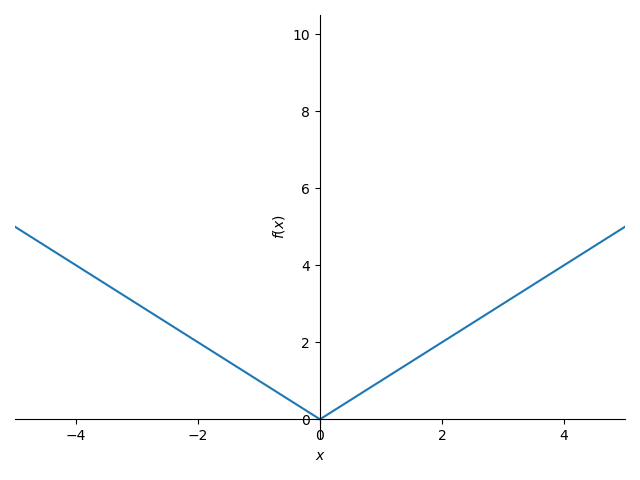
\includegraphics[width=10.5cm]{abs_simbol.png}
		\bicaption{Representacion de la funcion $f(x)  = |x|$ entre $-5$ y $5$}{Function $f(x) = |x|$ into the interval $(-5,5)$ } \label{fig:simplot1}
\end{figure}
\begin{paracol}{2}
El resultado se muestra en la figuras \ref{fig:simplot1}

Es posible también representar curvas paramétricas, $x(t),\ y(t)$, mediante el empleo del comando \mintinline{python}|plot_parametric|. Como por ejemplo, $x(t) = t\cos(t),\  y(t)= t\sin(t)$ representa una espiral en el plano $x,\ y$. Para obtener su gráfica se debe pasar  las funciones simbólicas $x(t)$ e $y(t)$ en una tupla y a continuación la variable simbólica que represente el parámetro, $t$, y el intervalo de valores del parámetro $[t_{min} \ t_{max}]$ para los que se quiere obtener la gráfica.  El siguiente código muestra cómo obtener la representación gráfica de la curva paramétrica $x(t),y(t)$ del ejemplo anterior.
\switchcolumn
The result is shown in figure \ref{fig:simplot1}

It is also possible to represent parametric functions, $x(t),\ y(t)$. To do it, we  use the command \mintinline{python}|plot_parametric|. For example, $x(t) = t\cos(t),\  y(t)= t\sin(t)$ represent a spiral on the $x,\ y$ plane. To plot in we should pass to the function the symbolic functions $x(t)$ and $y(t)$ into a tuple followed by the symbolic variable that represent the parameter, $t$, and the interval of parameter values $[t_{min} \ t_{max}]$ for which we want to draw the plot. The following code shows how to get the graphic representation of the previous example, $x(t),y(t)$, parametric function. 
\end{paracol}
\begin{center}
	\begin{minipage}{.6\textwidth}
		\begin{minted}{python}
In [60]: t = sp.symbols('t')
In [61]: x = t*sp.cos(t)
In [62]: y = t*sp.sin(t)
In [63]: dr = sp.plot_parametric((x,y),(t,0,10))
In [64]: dr.xlabel='x'
In [65]: dr.ylabel='y'
In [66]: dr[0].line_color= 'red'
In [67]: dr.show()
		\end{minted}
	\end{minipage}
\end{center}
\begin{paracol}{2}
En este caso, además hemos creado un objeto grafico \mintinline{python}|dr|, de modo que podemos después modificar las propiedades del gráfico, usando los mismos comando que emplearíamos en Matplotlib. Destacar el uso de \mintinline{python}|dr.show()| para actualizar el gráfico con los parámetros modificados. El resultado final se muestra en la figura \ref{fig:simplot1}.
\switchcolumn
In this case, we have also created a graphic object \mintinline{python}|dr|, which will allow us to modify the graphics properties later on using the same commands we would use with Matplotlib. It is interesting to notice that use of \mintinline{python}|dr.show()| to update the figure with the modified parameters. The final result is shown in figure \ref{fig:simplot1}.
\end{paracol}
 
\begin{figure}
	\centering
	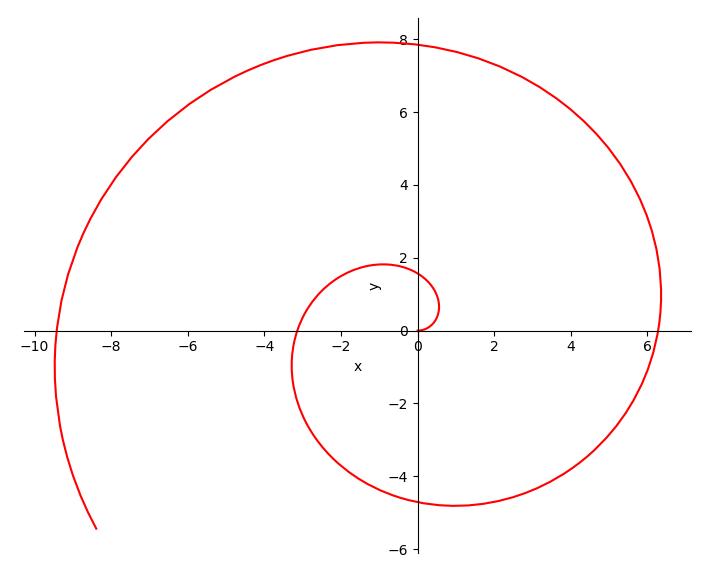
\includegraphics[width=10.5cm]{espiral.png}
	\bicaption{Gráfica de la curva paramétrica $x(t) = t\cos(t), y(t)= t\sin(t)$ obtenida a partir de su expresión simbólica.}{Graphic of parametric function $x(t) = t\cos(t), y(t)= t\sin(t)$ drawn from its symbolic expression}
		\label{fig:simpar}
		
\end{figure}
 

\begin{paracol}{2} 
Una aplicación directa de la representación de curvas paramétricas es la obtención de la trayectoria de un móvil conocida su posición en función del tiempo. Por ejemplo, la obtención de la parábola trazada por un cuerpo que se mueve bajo la fuerza de la gravedad. 


Por último es también posible representar superficies empleando funciones simbólicas de dos variables. Para ello se emplea el comando \texttt{plot3d}. En este caso, es preciso suministrarle al menos la función de dos variables que se desea representar. Si no se especifica rango, Sympy por defecto representará la función en el intervalo $(-10,10)$, tanto para el eje x como para  como para el y. Además, \texttt{plot3d} admite tuplas de tres elementos $(x, x_{min}, x_{max})$  $()y, y_{min},y_{max})$ que indica el área sobre la que se quiere representar la función. Es posible también añadir parámetros,\\ \mintinline{python}|nb_of_points_x=100,nb_of_points_y=100|\\  al comando que especifican el tamaño de la retícula empleada para representar la superficie. 
\switchcolumn
A simple application of parametric functions is plotting a mobile trajectory based on the position as a function of time. For example, this includes the plot of a parabola that represents a body moving under gravitational force.

Finally, it is possible to draw surfaces using symbolic functions of two variables. We use the command \texttt{plot3d} to do this. To use this command, it is necessary to provide at least the two-variable function that we want to visualize. If we do not specify a range, SymPy represents the function in the interval \((-10, 10)\) for both the x and y axes. 

Additionally, \texttt{plot3d} accepts three-element tuples \((x, x_{\text{min}}, x_{\text{max}})\) and \((y, y_{\text{min}}, y_{\text{max}})\) to indicate the area over which you want to draw the function. You can also add parameters such as\\ \mintinline{python}|nb_of_points_x=100,nb_of_points_y=100|\\ to the command to specify the size of the mesh used to represent the surface.
\end{paracol}  
\begin{center}
	\begin{minipage}{.9\textwidth}
		\begin{minted}{python}
In [124]: x,y = sp.symbols('x y')
In [125]: f3 = sp.sin(sp.sqrt(x**2+y**2))
In [126]: f3
Out[126]: 
		\end{minted}
		$\sin(\sqrt{x^2+y^2})$
		\begin{minted}{python}
In [127]: sp.plotting.plot3d(f3,(x,-2*sp.pi,2*sp.pi),(y,-2*sp.pi,2*sp.pi),
nb_of_points_x=100,nb_of_points_y=100)
Out[127]: <sympy.plotting.plot.Plot at 0x798926f7c610>
		\end{minted}
	\end{minipage}
\end{center}
\begin{paracol}{2}
La figura \ref{fig:surfsim} muestra los resultados de este ejemplo.
\switchcolumn
Figure \ref{fig:surfsim} shows the results of this example.
\end{paracol}
\begin{figure}[h]
\centering
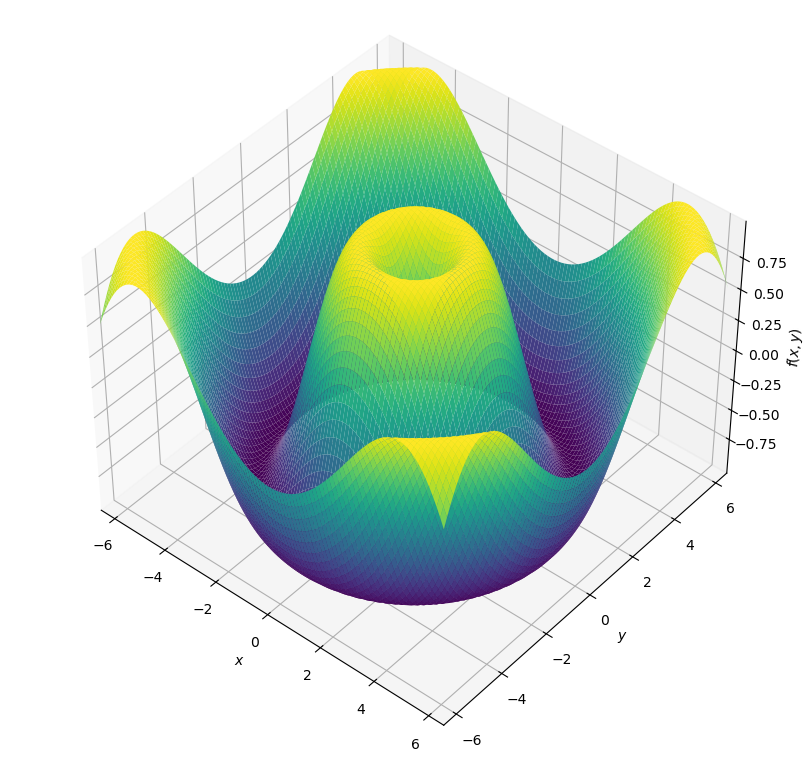
\includegraphics[scale=0.5]{sim_3d.png}
\caption{Gráfica de la función $f(x) = \sin\left(\sqrt{x^2+y^2}\right)$ obtenida a partir de su expresión simbólica con el comando \texttt{ezsurf} de Matlab }
\label{fig:surfsim}
\end{figure}
\begin{paracol}{2}
Hasta aquí la introducción al cálculo simbólico. Para obtener una visión completa de sus posibilidades es imprescindible consultar la documentación de Sympy.
\switchcolumn
So far, the introduction to symbolic computing. In order to get a complete vision of its possibilities it is mandatory to check the Sympy documentation 
\end{paracol}
\begin{flalign*}
	&&\biggr \}\reversemathwitch* 
\end{flalign*}




  

  	 